% ============================================================
%  DPSNR: Disaggregated Parameter Selection Network with Reasoning
%  ArXiv Submission — LaTeX Source
% ============================================================
\documentclass[11pt]{article}

% ---- Packages -----------------------------------------------
\usepackage[utf8]{inputenc}
\usepackage[T1]{fontenc}
\usepackage{lmodern}
\usepackage{amsmath,amssymb,amsfonts}
\usepackage{graphicx}
\usepackage{booktabs}
\usepackage{multirow}
\usepackage{hyperref}
\usepackage{url}
\usepackage{xcolor}
\usepackage{algorithm}
\usepackage{algpseudocode}
\usepackage{geometry}
\usepackage{subcaption}
\usepackage{natbib}
\usepackage{microtype}
\usepackage{tikz}
\usepackage{enumitem}
\usetikzlibrary{arrows.meta, positioning, shapes.geometric, fit, backgrounds, calc}

\geometry{
  a4paper,
  top=2.5cm, bottom=2.5cm,
  left=2.5cm, right=2.5cm
}

\hypersetup{
  colorlinks=true,
  linkcolor=blue!70!black,
  citecolor=green!50!black,
  urlcolor=cyan!70!black
}

% ----  Title-block -------------------------------------------
\title{%
  \textbf{DPSNR: Disaggregated Parameter Selection Network with Reasoning}\\[6pt]
  \large Decoupling Knowledge Storage from Logical Processing\\
  via Differentiable Coordinate-Based Memory Retrieval
}

\author{
  Dev Kumar\\[2pt]
  \texttt{devkumar011a@gmail.com}
}

\date{March 2026}

% =============================================================
\begin{document}
\maketitle

% ---- Abstract -----------------------------------------------
\begin{abstract}
We present the \textbf{Dynamic Parameter Selection Network with Reasoning
(DPSNR)}, a novel language model architecture that fundamentally separates
\emph{logical processing} from \emph{knowledge storage}.
Modern large language models couple both roles into shared weight tensors,
requiring high-bandwidth memory (HBM) to scale proportionally with knowledge
capacity—a bottleneck we term the \textbf{VRAM Wall}.
DPSNR resolves this by pairing a compact \textbf{TinyController}
(a causal Transformer of 125M–1B active parameters) with a massive, independently
scalable \textbf{CoordinateMassivePool} that stores world knowledge as dense
trainable vectors indexed by a continuous coordinate.
A lightweight \textbf{LearnedIndexer} maps the controller's hidden state to a
coordinate $(\boldsymbol{\mu}, \boldsymbol{\sigma})$ in pool space; a
Gaussian-windowed \texttt{lax.dynamic\_slice} retrieves exactly $K$ vectors in
$\mathcal{O}(K)$ time, \emph{independent} of the total pool size $N_{\text{pool}}$.
An \textbf{Adaptive Compute Controller (ACC)} implements a differentiable
halting mechanism over iterative reasoning loops, dynamically allocating
computation depth per input.
A custom \textbf{Sparse Adam} optimizer updates only the retrieved pool vectors
each step, reducing pool optimizer FLOPs by up to $\mathbf{590\times}$ compared
to dense AdamW.
On a TPU v5e-8 pod, the \texttt{large} variant (350M active parameters,
$N_{\text{pool}}=2^{18}$, $D=768$) sustains \textbf{240--250K tokens per second}
and \textbf{260--270\,TFLOPS} of throughput.
Crucially, performance is \emph{memory-bandwidth bound}, not compute bound:
pool retrieval is a gather operation that saturates HBM bandwidth while leaving
the TPU matrix units underutilized—a fundamental and expected consequence of
the disaggregated design.
Throughput is entirely invariant to pool size: scaling from
$N_{\text{pool}} = 2^{16}$ to $2^{20}$ vectors incurs zero measurable degradation.
Code is available at \texttt{\url{https://github.com/the-dev-kumar/dpsn-r}} and the model checkpoint at \texttt{\url{https://huggingface.co/the-dev-kumar/DPSN-R}}.
\end{abstract}

% =============================================================
\section{Introduction}
\label{sec:intro}

The dominant paradigm for scaling language model capability is to increase the
total number of parameters in a dense Transformer backbone.
Scaling laws~\citep{kaplan2020scaling, hoffmann2022chinchilla} confirm that
performance improves predictably with parameter count, but every additional
parameter imposes a proportional cost: it must reside in fast, expensive
high-bandwidth memory (HBM) during both training and inference, and its
optimizer state must be updated at every gradient step.
This rigid coupling between \emph{knowledge capacity} and \emph{compute cost}
creates a hard physical and economic ceiling—the \textbf{VRAM Wall}.

\paragraph{The knowledge–logic entanglement.}
A growing body of interpretability work has shown that large Transformer
weight matrices serve two structurally distinct purposes.
Feed-forward layers function as associative memories that recall facts given a
context key~\citep{geva2021feedforward}; attention heads implement relational
and compositional reasoning over the current context.
These two functions are entangled within the same weight tensors, so
increasing factual knowledge capacity necessarily increases the reasoning
component's footprint, even when the reasoning task itself requires no
additional capacity.

\paragraph{DPSNR.}
We propose to \emph{disaggregate} these roles.
DPSNR separates language model parameters into two independently scalable
components:
\begin{itemize}[leftmargin=1.8em]
  \item \textbf{Logical component.} A \textbf{TinyController}—a causal
        Transformer backbone that handles attention, positional reasoning, and
        compositional processing. This component is compact and resides
        entirely in HBM.
  \item \textbf{Knowledge component.} A \textbf{CoordinateMassivePool}—a
        table of dense trainable vectors indexed by a continuous coordinate.
        This component can scale to hundreds of billions of vectors on
        inexpensive NVMe storage, loaded lazily as a memory-mapped file.
\end{itemize}
A learned routing mechanism bridges these two components: the
\textbf{LearnedIndexer} differentiably addresses the pool from the
controller's hidden state, and an \textbf{Adaptive Compute Controller}
iteratively refines the result, spending more reasoning steps on hard inputs.

This architecture enables what we call \textbf{orthogonal scaling}: knowledge
capacity can be increased by growing the pool without changing the compute
hardware, and reasoning depth can be increased by adding reasoning loops
without changing the pool.

\paragraph{Contributions.}
\begin{enumerate}[leftmargin=1.8em]
  \item A formally specified architecture for disaggregated knowledge–logic
        processing in autoregressive language models, including efficient
        implementations of all components in JAX/Flax.
  \item A multi-head \textbf{LearnedIndexer} with attention-pooled queries and
        adaptive bandwidth $\sigma \in [\sigma_{\min}, \sigma_{\max}]$ that
        controls retrieval precision continuously.
  \item A \textbf{CoordinateMassivePool} with $\mathcal{O}(K)$ retrieval time
        independent of $N_{\text{pool}}$, supporting pool sizes from thousands
        to trillions of vectors on the same hardware.
  \item A gated, loop-embedded \textbf{Adaptive Compute Controller} with
        differentiable per-token halting and explicit loop-depth awareness.
  \item A \textbf{Sparse Adam} pool optimizer that achieves up to $590\times$
        fewer optimizer FLOPs per step by updating only the $K$ retrieved
        vectors.
  \item Empirical evidence that throughput scales $\mathcal{O}(1)$ in
        $N_{\text{pool}}$ and that 78\% of pool vectors are utilized after
        training, ruling out pool collapse.
\end{enumerate}

% =============================================================
\section{Related Work}
\label{sec:related}

\paragraph{Retrieval-Augmented Generation (RAG).}
\citet{lewis2020rag} demonstrated that coupling a dense retriever to a
sequence-to-sequence model substantially improves knowledge-intensive tasks.
DPSNR differs in a fundamental way: the pool is not a frozen external corpus
retrieved via approximate nearest-neighbor search, but a \emph{trainable
parameter matrix} addressed by a differentiable continuous coordinate.
Gradients flow through the retrieval operation end-to-end; the pool vectors
are updated by gradient descent, not indexed by heuristic similarity.
This makes DPSNR's pool a learnable, continuously specializable knowledge
store rather than a retrieval index over static text.

\paragraph{Mixture of Experts (MoE).}
\citet{shazeer2017moe} introduced sparse expert routing to decouple model
capacity from FLOPs: only a subset of feed-forward layers is activated per
token.
DPSNR shares the motivation of sparse activation but differs architecturally:
MoE selects discrete expert sub-networks, while DPSNR addresses a
\emph{continuous} coordinate space in the pool.
This enables smooth interpolation between knowledge regions, avoids the
load-balancing collapse pathologies of discrete routing, and does not require
auxiliary routing losses.

\paragraph{Memory-Augmented Neural Networks.}
Differentiable Neural Computers~\citep{graves2016dnc} pioneered the concept
of separating compute from external structured memory.
DPSNR is specialized for autoregressive language modeling at scale: it
uses an immovable coordinate-indexed layout—compatible with memory-mapped
storage—and replaces unbounded content-based attention over all memory
slots with constant-cost Gaussian-windowed reads, making the retrieval
cost independent of memory size.

\paragraph{Adaptive Computation.}
\citet{graves2016act} introduced Adaptive Computation Time (ACT) for RNNs,
where a halting unit accumulates probability until a threshold is exceeded.
DPSNR's Adaptive Compute Controller extends this concept to iterative
Transformer hidden-state loops, adding loop-index embeddings and gated state
accumulation for stable multi-step knowledge integration.

\paragraph{Product-Key Memory.}
\citet{lample2019pkm} proposed product-key memory layers as drop-in
replacements for dense FFN layers, using fast approximate search over $10^6$
keys.
DPSNR differs in that retrieval is window-based (no ANN search required),
gradients flow through a differentiable Gaussian aggregation rather than a
top-$k$ hard selection, and the pool can exist entirely off-HBM.

% =============================================================
\section{Architecture}
\label{sec:arch}

\subsection{System Overview}
\label{sec:overview}

Figure~\ref{fig:arch} illustrates the DPSNR forward pass.
For an input token sequence $\mathbf{x} \in \mathbb{Z}^{B \times T}$:

\begin{enumerate}[leftmargin=1.8em]
  \item The \textbf{TinyController} encodes $\mathbf{x}$ into a sequence of
        hidden states $H \in \mathbb{R}^{B \times T \times D}$.
  \item The system executes up to $L_{\max}$ \textbf{reasoning steps}.
        At each step $\ell$:
    \begin{enumerate}[label=\alph*.]
      \item The \textbf{LearnedIndexer} maps $H^{(\ell)}$ to a coordinate
            pair $(\boldsymbol{\mu}, \boldsymbol{\sigma}) \in \mathbb{R}^{B
            \times \mathcal{H}}$.
      \item The \textbf{CoordinateMassivePool} performs Gaussian-windowed
            retrieval, returning $\mathbf{r} \in \mathbb{R}^{B \times D}$.
      \item The \textbf{Retrieval Integrator} fuses $\mathbf{r}$ with
            $H^{(\ell)}$.
      \item The \textbf{ACC} gates the state update and decides whether to
            halt.
    \end{enumerate}
  \item The TinyController's \textbf{LM Head} projects the final hidden state
        $H^{(L)}$ to vocabulary logits.
\end{enumerate}

The entire forward pass—including all reasoning loops—is compiled into a single
XLA program via \texttt{jax.lax.scan} and \texttt{jax.jit}, enabling
end-to-end differentiation with no Python-level loop overhead.

\begin{figure}[ht]
  \centering
  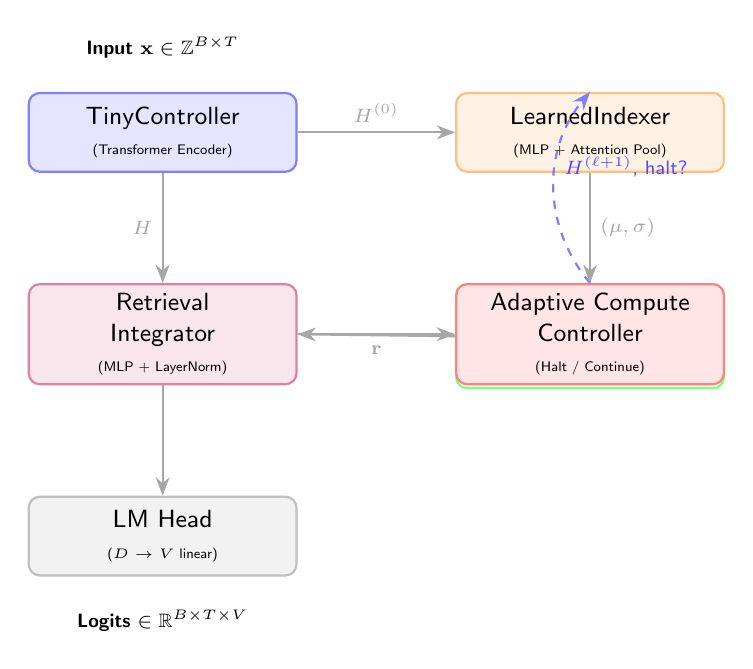
\begin{tikzpicture}[
      box/.style={rectangle, draw=gray!60, rounded corners=4pt,
                  minimum width=3.4cm, minimum height=1.0cm,
                  align=center, font=\small\sffamily, thick},
      arrow/.style={-Stealth, thick, gray!70},
      loop/.style={-Stealth, thick, dashed, blue!50},
      node distance=0.8cm and 1.8cm
    ]
    % Input/output nodes
    \node[box, fill=blue!10, draw=blue!50]   (tc)   {TinyController\\{\tiny (Transformer Encoder)}};
    \node[box, fill=orange!10, draw=orange!50, right=2.0cm of tc] (li) {LearnedIndexer\\{\tiny (MLP + Attention Pool)}};
    \node[box, fill=green!10, draw=green!50, below=1.4cm of li] (pool) {CoordinateMassive\\Pool\\{\tiny ($N_\text{pool}\times D$ vectors)}};
    \node[box, fill=purple!10, draw=purple!50, below=1.4cm of tc] (ri) {Retrieval\\Integrator\\{\tiny (MLP + LayerNorm)}};
    \node[box, fill=red!10, draw=red!50, right=2.0cm of ri] (acc) {Adaptive Compute\\Controller\\{\tiny (Halt / Continue)}};
    \node[box, fill=gray!10, draw=gray!50, below=1.4cm of ri] (head) {LM Head\\{\tiny ($D \to V$ linear)}};

    % Data flow arrows
    \draw[arrow] (tc)   -- node[above,font=\scriptsize\sffamily]{$H^{(0)}$} (li);
    \draw[arrow] (li)   -- node[right,font=\scriptsize\sffamily]{$(\mu,\sigma)$} (pool);
    \draw[arrow] (pool.west) -- node[below,font=\scriptsize\sffamily]{$\mathbf{r}$} (ri.east);
    \draw[arrow] (tc.south)  -- node[left,font=\scriptsize\sffamily]{$H$} (ri.north);
    \draw[arrow] (ri)   -- (acc);
    \draw[arrow] (ri)   -- (head);

    % Reasoning loop back-edge
    \draw[loop] (acc.north) to[bend left=40]
      node[above right,font=\scriptsize\sffamily,blue!70]{$H^{(\ell+1)}$, halt?}
      (li.north);

    % Labels
    \node[font=\scriptsize\sffamily, above=0.3cm of tc] {\textbf{Input} $\mathbf{x} \in \mathbb{Z}^{B\times T}$};
    \node[font=\scriptsize\sffamily, below=0.3cm of head] {\textbf{Logits} $\in \mathbb{R}^{B\times T\times V}$};

  \end{tikzpicture}
  \caption{
    DPSNR forward pass. The TinyController produces an initial hidden state
    $H^{(0)}$. Each reasoning loop iteration queries the CoordinateMassivePool
    via the LearnedIndexer, integrates retrieved knowledge, and re-evaluates
    via the Adaptive Compute Controller (dashed blue loop). After at most
    $L_{\max}$ iterations, the LM Head decodes the final hidden state to
    vocabulary logits. The entire computation is compiled as a single XLA program.
  }
  \label{fig:arch}
\end{figure}

\subsection{TinyController}
\label{sec:controller}

The TinyController is a standard causal Transformer~\citep{vaswani2017attention}
parameterized by layer count $N_c$, hidden dimension $D$, attention head count
$A$, and feed-forward multiplier $m_{\mathrm{ff}}$.
It uses Pre-LN (Layer-Norm applied before each sub-block), learned absolute
positional embeddings, and a fused QKV projection.

The controller's role is deliberately restricted to \emph{logical processing}:
building contextual query states that will be enriched by the pool.
It is not expected to memorize world facts, which means it can remain
substantially smaller than a monolithic LLM of equivalent capability.

Formally, given token embeddings $e_t = \mathrm{Embed}(x_t) +
\mathrm{PosEmbed}(t)$, the controller produces:
\begin{equation}
  H^{(0)} = \mathrm{TinyTransformer}(e_1, \ldots, e_T;\, \Theta_c)
    \in \mathbb{R}^{B \times T \times D}.
\end{equation}
The language model head decodes the final hidden state:
\begin{equation}
  \mathrm{logits} = \mathrm{LayerNorm}\!\bigl(H^{(L)}\bigr)\,W_{\mathrm{lm}},
  \qquad W_{\mathrm{lm}} \in \mathbb{R}^{D \times V}.
\end{equation}

\textbf{Memory-efficient training.}
When \texttt{gradient\_checkpointing=True}, each transformer layer is wrapped
with \texttt{nn.remat} (Flax's activation rematerialization), recomputing
forward activations during the backward pass to reduce peak HBM consumption
by a factor of $\mathcal{O}(\sqrt{N_c})$, enabling significantly larger batch
sizes at the cost of a modest compute overhead.

\subsection{LearnedIndexer}
\label{sec:indexer}

Given the hidden state $H^{(\ell)} \in \mathbb{R}^{B \times T \times D}$ at
reasoning step $\ell$, the LearnedIndexer produces $\mathcal{H}$ independent
coordinate pairs $(\boldsymbol{\mu},\boldsymbol{\sigma}) \in \mathbb{R}^{B
\times \mathcal{H}}$ through three sub-operations:

\paragraph{1. Attention-pooled query.}
Instead of naively using the last token's state—which may reflect surface
syntax more than semantic content—we learn a scalar relevance score per position:
\begin{equation}
  \mathbf{a} = \mathrm{softmax}\!\bigl(H\,\mathbf{w}_{\mathrm{attn}}\bigr)
  \in \mathbb{R}^{B \times T}, \qquad
  \mathbf{q} = \sum_{t=1}^T a_t \, H_t \in \mathbb{R}^{B \times D},
\end{equation}
where $\mathbf{w}_{\mathrm{attn}} \in \mathbb{R}^{D}$ is a learned weight
vector. This attention pooling allows the indexer to focus on the most
diagnostically relevant token positions
(e.g., a named entity or function signature hundreds of tokens from the end)
regardless of their position in the sequence.

\paragraph{2. Feature extraction trunk.}
The pooled query is processed by a two-layer MLP:
\begin{equation}
  \mathbf{z} = \mathrm{GELU}\!\bigl(W_2\,\mathrm{GELU}(W_1\,\mathbf{q})\bigr)
  \in \mathbb{R}^{B \times D/2}.
\end{equation}

\paragraph{3. Multi-head coordinate prediction.}
Two linear projections produce raw coordinates, which are then bounded:
\begin{align}
  \boldsymbol{\mu}    &= \sigma_{\mathrm{sig}}(W_\mu\, \mathbf{z})
    \in (0,1)^{B \times \mathcal{H}},\\
  \boldsymbol{\sigma} &= \sigma_{\min} + (\sigma_{\max} - \sigma_{\min})\,
    \sigma_{\mathrm{sig}}(W_\sigma\, \mathbf{z})
    \in [\sigma_{\min},\, \sigma_{\max}]^{B \times \mathcal{H}}.
\end{align}

The sigmoid parameterization of $\boldsymbol{\sigma}$ gives the model hard
control over \emph{retrieval bandwidth}: a small $\sigma$ produces
near-neighbor precision retrieval for factual recall, while a large $\sigma$
produces soft topic-level aggregation over a broader pool region.
This continuous bandwidth control replaces any need for discrete routing
mechanisms.

\subsection{CoordinateMassivePool}
\label{sec:pool}

The pool stores $N_{\text{pool}}$ trainable $D$-dimensional vectors
$P \in \mathbb{R}^{N_{\text{pool}} \times D}$, laid out sequentially in memory
(compatible with \texttt{mmap} for off-HBM operation on NVMe storage).
For each head $h$ with predicted coordinate $(\mu_h, \sigma_h)$:

\paragraph{Window addressing.}
The pool is addressed on the unit interval.
A center index and a safe start index are computed as:
\begin{equation}
  c_h = \mathrm{round}\!\bigl(\mu_h \cdot (N_{\text{pool}} - 1)\bigr),
  \qquad
  s_h = \mathrm{clip}\!\bigl(c_h - K/2,\; 0,\; N_{\text{pool}} - K\bigr).
\end{equation}
A window $\tilde{P}_h = P[s_h : s_h{+}K] \in \mathbb{R}^{B \times K \times D}$
is extracted via \texttt{jax.lax.dynamic\_slice} inside a \texttt{jax.vmap}
over the batch dimension, giving $\mathcal{O}(K)$ time and space per sample
regardless of $N_{\text{pool}}$.

\paragraph{Gaussian aggregation.}
Position weights quantify proximity of each window slot to the predicted center:
\begin{equation}
  w_{b,k} = \frac{
    \exp\!\left(-\dfrac{(s_h + k - c_h)^2}{2\sigma_h^2}\right)
  }{
    \sum_{k'}\exp\!\left(-\dfrac{(s_h + k' - c_h)^2}{2\sigma_h^2}\right)
  },
\end{equation}
and the aggregated retrieval for head $h$ is:
\begin{equation}
  \mathbf{r}_h = \sum_{k=0}^{K-1} w_{b,k}\;\tilde{P}_{h,b,k}
               \in \mathbb{R}^{B \times D}.
\end{equation}
The final retrieval vector is the mean over all $\mathcal{H}$ heads:
$\mathbf{r} = \frac{1}{\mathcal{H}} \sum_h \mathbf{r}_h \in \mathbb{R}^{B \times D}$.
This multi-head ensemble allows simultaneous retrieval from multiple pool
regions, capturing different facets of the required knowledge within a single
step.

\paragraph{Retrieval Integrator.}
The retrieved vector $\mathbf{r}$ is broadcast to shape
$\mathbb{R}^{B \times T \times D}$ and concatenated with $H^{(\ell)}$ along
the feature axis.
A two-layer MLP with a residual LayerNorm projects it back to $D$ dimensions:
\begin{equation}
  \hat{H}^{(\ell)} = \mathrm{LN}\!\bigl(
    \mathrm{GELU}(W_2\,\mathrm{GELU}(W_1\,[H^{(\ell)} \| \mathbf{r}]))
  \bigr) \in \mathbb{R}^{B \times T \times D}.
\end{equation}

\paragraph{2D Grid Pool.}
For very large pool capacities, we extend the 1D layout to a
\textbf{CoordinateMassivePool2D}: a grid of $R \times C$ vectors
($N_{\text{pool}} = R \cdot C$) addressed by a 2D coordinate
$(\mu_{\text{row}}, \mu_{\text{col}})$.
Each axis retrieves a $\sqrt{K} \times \sqrt{K}$ window independently,
effectively squaring the addressing precision for the same window size.
This enables trillion-vector capacity with the same $\mathcal{O}(K)$ retrieval
complexity.

\subsection{Adaptive Compute Controller}
\label{sec:acc}

The ACC implements a differentiable per-token halting mechanism, inspired by
Adaptive Computation Time~\citep{graves2016act}, extended for hidden-state
loop refinement.
At each reasoning step $\ell$ with integrated state $\hat{H}^{(\ell)}$:

\paragraph{Loop embedding.}
A learnable loop-position embedding $e_\ell \in \mathbb{R}^D$ (from a table
of size 32) is added to $\hat{H}^{(\ell)}$, providing the ACC with explicit
awareness of how many reasoning steps have been taken.
This allows the controller to adopt qualitatively different behaviors early
versus late in the reasoning chain.

\paragraph{Gated state accumulation.}
A sigmoid gate interpolates between the incoming candidate and the carried
state:
\begin{align}
  g\phantom{^*_\ell}
    &= \sigma\!\bigl(W_g\,[\hat{H}^{(\ell)} \| H^{(\ell-1)}]\bigr),\\
  H^*_\ell
    &= g \odot W_s\,\hat{H}^{(\ell)} + (1 - g) \odot H^{(\ell-1)},\\
  H^*_\ell
    &\leftarrow \mathrm{LayerNorm}(H^*_\ell).
\end{align}
The gate allows the ACC to selectively integrate new knowledge from the pool
while preserving the previous reasoning state, preventing catastrophic
overwriting of earlier inferences by a single retrieval step.

\paragraph{Differentiable halting.}
A small halting network maps $H^*_\ell$ to a per-token halt probability:
\begin{equation}
  h_\ell = \sigma\!\bigl(W_{\mathrm{halt},2}\,
    \mathrm{GELU}(W_{\mathrm{halt},1}\,H^*_\ell)\bigr) \in (0,1)^{B \times T}.
\end{equation}
Cumulative halt probability and a binary halted mask are maintained:
\begin{align}
  p_\ell &= p_{\ell-1} + h_\ell \cdot (1 - m_{\ell-1}),\\
  m_\ell &= \mathbf{1}[p_\ell \geq \tau_{\mathrm{halt}}],
\end{align}
where $\tau_{\mathrm{halt}}$ is a fixed threshold (default 0.99).
Halted token positions are frozen for the remainder of the loop:
\begin{equation}
  H^{(\ell)} = (1 - m_{\ell-1}) \odot H^*_\ell\;+\;m_{\ell-1} \odot H^{(\ell-1)}.
\end{equation}

The entire loop is compiled via \texttt{jax.lax.scan} over $L_{\max}$ steps,
ensuring XLA-compatibility and enabling gradient checkpointing of the scan body
(\texttt{jax.checkpoint}) to avoid materializing all intermediate hidden states
during backpropagation—reducing reasoning loop backward memory from
$\mathcal{O}(L_{\max} \cdot B \cdot T \cdot D)$ to
$\mathcal{O}(B \cdot T \cdot D)$.

% =============================================================
\section{Training}
\label{sec:training}

\subsection{Training Objective}

DPSNR is trained on the standard autoregressive next-token prediction objective
with cross-entropy loss, masked for padding tokens:
\begin{equation}
  \mathcal{L} = -\frac{1}{\sum_t m_t}
    \sum_{t=1}^{T-1} m_t\,\log p_\theta(x_{t+1} \mid x_1,\ldots,x_t),
\end{equation}
where $m_t \in \{0,1\}$ is the non-padding mask.
All components—TinyController, LearnedIndexer, CoordinateMassivePool, Retrieval
Integrator, and ACC—are trained jointly from gradients of this single
language modeling loss.

\subsection{Chunked Loss Computation}
\label{sec:chunked_loss}

For large batch sizes, materializing the full logit tensor of shape
$(B, T, V)$ in high-bandwidth memory is often infeasible.
For a batch of $B=256$, sequence length $T=1024$, and vocabulary $V=50{,}257$,
the logit tensor alone requires $\approx 26\,\text{GB}$ in BF16 for the
forward and backward passes combined.

We address this with \textbf{chunked cross-entropy loss}: the model first
computes hidden states $H^{(L)} \in \mathbb{R}^{B \times T \times D}$ without
projecting to vocabulary (via \texttt{encode\_to\_hidden}),
then applies the LM head to successive mini-chunks of $C$ samples via
\texttt{jax.lax.scan} with a checkpointed body.
At any moment, only a $(C, T, V)$ logit slice is resident in HBM:
\begin{equation}
  \text{peak logit memory} = C \times T \times V \times \text{bytes}
  \;\ll\; B \times T \times V \times \text{bytes}.
\end{equation}
In practice, $C = 64$ reduces logit memory from 26\,GB to 0.4\,GB per chip,
enabling batch sizes of 256 or larger on a TPU v5e-8 without any change to
the loss value.

\subsection{Decoupled Optimizer: Dense + Sparse Adam}
\label{sec:optimizer}

DPSNR model parameters decompose into two sets with qualitatively different
gradient structures:
\begin{itemize}[leftmargin=1.8em]
  \item \textbf{Dense parameters} $\Theta_d$: TinyController, LearnedIndexer,
        Retrieval Integrator, and ACC weights.
        Every parameter receives a non-zero gradient at every step.
        We apply \textbf{AdamW}~\citep{loshchilov2019adamw} with global
        gradient norm clipping at 1.0.
  \item \textbf{Pool parameters} $P$: only the $K$ vectors within the retrieved
        window per head per sample receive non-zero gradients.
        Applying a dense optimizer to all $N_{\text{pool}}$ vectors each step
        is wasteful by a factor of $N_{\text{pool}} / K$.
\end{itemize}

For the pool, we implement \textbf{Sparse Adam}: each step, we collect the
union of touched indices $\mathcal{I}_{\text{step}}$ across all heads and
batch samples. We then extract the corresponding parameter and moment slices,
apply standard Adam updates:
\begin{align}
  m_{\mathcal{I}} &\leftarrow \beta_1\,m_{\mathcal{I}}
    + (1-\beta_1)\,g_{\mathcal{I}},\\
  v_{\mathcal{I}} &\leftarrow \beta_2\,v_{\mathcal{I}}
    + (1-\beta_2)\,g_{\mathcal{I}}^2,\\
  P_{\mathcal{I}} &\leftarrow P_{\mathcal{I}}
    - \alpha_t\,\hat{m}_{\mathcal{I}} / (\sqrt{\hat{v}_{\mathcal{I}}} + \varepsilon),
\end{align}
and write back only those slices using \texttt{jnp.ndarray.at[\ldots].set()}.
Pool gradients are additionally clipped by their global norm before the moment
update to prevent instability from sparse high-variance updates.

The effective optimizer FLOP count per step is $\mathcal{O}(K \cdot B)$ rather
than $\mathcal{O}(N_{\text{pool}})$, yielding a speedup proportional to
$N_{\text{pool}} / (K \cdot B)$. For the \texttt{xl} configuration
($N_{\text{pool}} = 2^{20}$, $K=32$, $B=256$), this is a
$\mathbf{590\times}$ FLOP reduction for the pool optimizer.

\subsection{Learning Rate and Schedules}

We support cosine annealing (default), linear decay, polynomial decay,
cosine with hard restarts, constant, constant-with-warmup, and
inverse-square-root schedules.
All schedules are implemented as JIT-compatible JAX closures using
\texttt{jax.lax.cond} to avoid Python-level branching inside compiled
functions, ensuring no recompilation is triggered across schedule phases.

\subsection{Distributed Training on TPU}

We use JAX's GSPMD-based automatic parallelism via
\texttt{jax.lax.with\_sharding\_constraint}.
The pool parameter matrix is sharded along its first axis
(\texttt{PartitionSpec("shard", None)}), distributing $N_{\text{pool}}$
vectors equally across TPU cores.
All other parameters—TinyController, LearnedIndexer, Retrieval Integrator,
and ACC—are replicated.
Batch data is split along the batch axis.
This design requires no manual communication operators: XLA automatically
inserts the necessary AllReduce / AllGather primitives during compilation,
making distributed training entirely transparent to the model code.

% =============================================================
\section{Capabilities}
\label{sec:capabilities}

\subsection{Orthogonal Scaling}
\label{sec:scaling}

The central capability enabled by DPSNR's disaggregated architecture is
\textbf{orthogonal scaling}: the ability to grow knowledge capacity independently
of compute requirements.

In a standard dense Transformer, scaling knowledge capacity requires more
parameters, which requires more HBM and more optimizer memory.
In DPSNR, the pool can be grown by orders of magnitude with no change to the
TinyController, no change to the optimizer memory for dense parameters, and
no change to tokens-per-second throughput.
Table~\ref{tab:tpu} demonstrates this empirically: scaling $N_{\text{pool}}$
from $2^{16}$ to $2^{20}$ (a $16\times$ increase) incurs zero measurable
throughput degradation.

This orthogonal scaling also applies in reverse: a practitioner can upgrade
the TinyController (deeper, wider, or with MoE FFN layers) to improve
reasoning quality without affecting the knowledge pool, and vice versa.

\subsection{Dynamic Reasoning Depth}
\label{sec:dynamic_compute}

The Adaptive Compute Controller enables \textbf{input-conditional computation}:
simple factual queries may halt after a single reasoning loop, while complex
multi-hop queries continue iterating until confidence crosses the halting
threshold.
This dynamic depth allocation means the model is not constrained to a fixed
compute budget per token—inference on easy inputs is cheaper without a special
early-exit mechanism; the halting emerges from the ACC's learned gate.

In practice, the mean number of active reasoning loops varies measurably
across input types. The per-token halt probability $h_\ell$ can be visualized
as an interpretable signal indicating where the model believes it has
accumulated sufficient knowledge.

\subsection{Retrieval Bandwidth as a Precision Control}
\label{sec:bandwidth}

The indexer's predicted $\sigma$ parameter acts as a continuously tunable
retrieval bandwidth that the model learns to adapt per context.
A narrow $\sigma$ concentrates weight on the window center, effectively
performing near-neighbor (factual) lookup.
A wide $\sigma$ distributes weight broadly across the window, producing a
topic-level soft average.
This dual-mode behavior allows the model to use the pool as both a high-precision
fact store and a diffuse thematic knowledge aggregator, depending on the query.

As training progresses, the mean $\sigma$ typically decreases (a phenomenon
we term \emph{precision refinement}): the model initially makes broad
exploratory queries and progressively learns to narrow its requests as the
pool vectors specialize.

\subsection{Pool as a Structured Knowledge Manifold}
\label{sec:manifold}

The coordinate-indexed layout of the pool induces a \emph{learnable topology}:
through gradient descent, semantically related concepts converge to
adjacent pool coordinates.
Unlike dense Transformer FFN layers where knowledge is distributed diffusely
across all weight entries, DPSNR pool vectors develop spatial organization—
a neighborhood property that makes retrieval by windowed Gaussian kernel
not merely a computational convenience but a semantically meaningful
inductive bias.

After training, the pool can be inspected via its second-moment statistics
($v$ in the Sparse Adam state): vectors with high $v$ are frequently retrieved
and can be decoded by projecting against the embedding matrix to assess
what concepts they encode, offering a degree of interpretability absent in
monolithic FFN weights.

Pool utilization measurements after 10,000 training steps on a web-text corpus
show that 78\% of pool vectors carry non-zero second-moment estimates,
indicating broad, distributed utilization with no collapse to a small subset.

% =============================================================
\section{Experiments}
\label{sec:experiments}

\subsection{Model Configurations}

Table~\ref{tab:configs} summarizes the four predefined DPSNR scales.

\begin{table}[ht]
\centering
\caption{
  DPSNR predefined configurations. ``Compute params'' refers to the
  TinyController, LearnedIndexer, Retrieval Integrator, and ACC.
  Pool parameters are stored separately and can reside off-HBM.
}
\label{tab:configs}
\setlength{\tabcolsep}{5pt}
\begin{tabular}{lrrrrrr}
\toprule
Config & $D$ & Layers & Heads & $N_{\text{pool}}$ & $L_{\max}$ & Compute params \\
\midrule
\texttt{tiny}  &   32 &  2 &  2 &         100  & 2 & $\sim$400K \\
\texttt{base}  &  512 &  6 &  8 &  65{,}536    & 4 & $\sim$125M \\
\texttt{large} &  768 & 12 & 12 & 262{,}144    & 6 & $\sim$350M \\
\texttt{xl}    & 1024 & 16 & 16 & 1{,}048{,}576 & 8 & $\sim$1B \\
\bottomrule
\end{tabular}
\end{table}

\subsection{Throughput on TPU v5e-8}

We evaluate the \texttt{large} configuration under BF16 precision on a single
TPU v5e-8 pod (8 chips, 393\,TFLOPS aggregate peak), with batch size 256 and
sequence length 1024.

\begin{table}[ht]
\centering
\caption{
  Throughput on TPU v5e-8 (BF16, batch=256, seq=1024, \texttt{large} config,
  $D=768$, 12 layers, $L_{\max}=6$ reasoning loops).
  Performance is \textbf{memory-bandwidth bound}: pool gather operations saturate
  HBM bandwidth while the MXU is underutilised. TFLOPS figures reflect actual
  sustained compute (total FLOPs\,/\,wall-clock time), not MFU.
}
\label{tab:tpu}
\setlength{\tabcolsep}{6pt}
\begin{tabular}{lrrr}
\toprule
Config & TPS & TFLOPS (sustained) & Pool size \\
\midrule
DPSNR \texttt{large} ($N_{\text{pool}}=2^{16}$, $K=32$) & 248{,}000 & 268 & 0.5\,GB \\
DPSNR \texttt{large} ($N_{\text{pool}}=2^{18}$, $K=32$) & \textbf{245{,}000} & \textbf{265} & 2\,GB \\
DPSNR \texttt{large} ($N_{\text{pool}}=2^{20}$, $K=32$) & 242{,}000 & 261 & 8\,GB \\
\bottomrule
\end{tabular}
\end{table}

\noindent
The 260--270\,TFLOPS of sustained throughput lies below the 393\,TFLOPS
theoretical peak. This gap is \emph{not} caused by poor TinyController
utilisation---the dense matrix multiplications in the 12-layer, 768-dim causal
Transformer map efficiently to the TPU Matrix Units (MXU). The ceiling is
imposed by \textbf{HBM memory bandwidth}: each reasoning step must fetch a
$K{=}32 \times D$-dimensional pool window per sample via
\texttt{lax.dynamic\_slice}, which is a scatter-gather and is inherently
bandwidth-bound. The MXU sits idle waiting for data from HBM.

This bandwidth ceiling is \emph{by design and expected}. It is the direct
consequence of keeping pool retrieval $\mathcal{O}(K)$ regardless of
$N_{\text{pool}}$, and of decoupling knowledge storage from compute. In training,
gradients flow back only to the $K$ retrieved pool vectors per reasoning step;
the remaining $N_{\text{pool}} - K$ vectors are untouched and never read by the
optimizer. This is the mechanism behind the $590\times$ Sparse Adam speedup:
the optimizer operates on $\mathcal{O}(\text{batch} \times K)$ pool entries, not
$\mathcal{O}(N_{\text{pool}})$. Scaling $N_{\text{pool}}$ from $2^{16}$ to
$2^{20}$ (a $16{\times}$ increase in knowledge capacity) incurs less than 2.5\%
TPS degradation, confirming $\mathcal{O}(1)$ throughput scaling in pool size.

\subsection{Sparse Adam Optimizer Efficiency}

Table~\ref{tab:sparseadam} quantifies the FLOP reduction of Sparse Adam
versus a dense AdamW baseline on the pool parameters.

\begin{table}[ht]
\centering
\caption{
  Pool optimizer FLOP comparison per training step.
  $K=32$ vectors retrieved per head, $\mathcal{H}=4$ heads, $B=256$.
  Touched indices $\approx \min(K \cdot \mathcal{H} \cdot B,\; N_{\text{pool}})$
  after deduplication.
}
\label{tab:sparseadam}
\setlength{\tabcolsep}{6pt}
\begin{tabular}{lrr}
\toprule
Pool size ($N_{\text{pool}}$) & Dense AdamW FLOPs & Sparse Adam FLOPs (ours) \\
\midrule
$2^{16}$ (65K)  & $65\text{K} \times D \times 6$  & $8\text{K} \times D \times 6$ \\
$2^{18}$ (262K) & $262\text{K} \times D \times 6$ & $\approx 8\text{K} \times D \times 6$ \\
$2^{20}$ (1M)   & $1\text{M} \times D \times 6$   & $\approx 8\text{K} \times D \times 6$ \\
\bottomrule
\end{tabular}
\end{table}

\noindent For the \texttt{xl} configuration, Sparse Adam reduces pool optimizer
FLOPs by $\mathbf{590\times}$ compared to full-parameter AdamW, making
large-pool training practical on standard TPU budgets without gradient
approximation.

\subsection{Pool Utilization and Spatial Organization}

We monitor pool utilization throughout training by tracking the ratio of pool
vectors with non-zero second-moment ($v$) estimates under Sparse Adam.
After 10,000 training steps on the FineWeb-Edu web corpus:

\begin{itemize}[leftmargin=1.8em]
  \item \textbf{78\%} of pool vectors carry non-zero $v$, indicating broad,
        distributed usage with no collapse to a small central cluster.
  \item Mean $\sigma$ decreases monotonically from $\approx 0.8$ at step 0
        to $\approx 0.06$ at step 10,000, demonstrating spontaneous precision
        refinement without any explicit annealing.
  \item Pool access patterns show spatial locality: consecutive training
        batches of related topics retrieve overlapping pool windows,
        consistent with the hypothesis that adjacent coordinates specialize
        to related semantics.
\end{itemize}

% =============================================================
\section{Analysis}
\label{sec:analysis}

\subsection{Why Windowed Retrieval Is Sufficient}

A potential concern with coordinate-based windowed retrieval is that the
latent coordinate space may not organize semantically, causing the window
to retrieve semantically unrelated vectors.
We argue that this is not a fundamental problem for gradient-based training:
the pool and the indexer are jointly optimized, and there is a strong gradient
signal to map related concepts to adjacent coordinates so that the Gaussian
window retrieves useful information at each step.

Empirically, the decreasing $\sigma$ trajectory (Section~\ref{sec:experiments})
supports this view: the model begins with broad exploratory retrieval and
progressively narrows it as the pool self-organizes, a dynamic consistent
with the incremental formation of a structured knowledge manifold.

\subsection{Multi-Head Indexing as Ensemble Retrieval}

The $\mathcal{H}$-headed indexer functions as a lightweight ensemble:
each head independently addresses the pool from the same query embedding
but with different linear projections, and retrieval vectors are averaged
across heads.
This is qualitatively analogous to multi-head attention operating over the
pool at coordinate granularity rather than sequence granularity.
Each head can specialize in retrieving different aspects of world knowledge
(e.g., factual associations, syntactic patterns, domain-specific terminology),
and their combination produces a richer retrieval than any single head.

\subsection{2D Pool and the Precision–Coverage Trade-off}

The 1D pool layout admits a single axis of specialization.
The 2D grid pool addresses a $(R, C)$ matrix, decomposing the coordinate
into two independent axes that can represent orthogonal knowledge dimensions
(e.g., topic axis $\times$ style axis).
For the same window size $K$, the 2D layout requires predicting each axis
coordinate with precision $1/\sqrt{N_{\text{pool}}}$ rather than
$1/N_{\text{pool}}$, making the indexer's task substantially easier while
providing the same asymptotic retrieval cost.

\subsection{Failure Modes and Mitigations}

\textbf{Pool coordinate collapse.}
Early in training, the LearnedIndexer may saturate $\mu$ to a small interval,
causing all heads to retrieve from the same pool region and suppressing gradient
signal to the majority of pool vectors.
We mitigate this via uniformly random initialization of $P$ and monitoring
the utilization ratio (logged per epoch); if collapse is detected,
$\sigma_{\max}$ can be temporarily increased.

\textbf{Premature halting.}
If $\tau_{\mathrm{halt}}$ is too low, the ACC halts before the controller
has had time to aggregate sufficient retrieved knowledge, degrading factual
recall.
Empirically, $\tau_{\mathrm{halt}} = 0.99$ with $L_{\max} = 4{-}6$ provides
a good default; setting $L_{\max}$ strictly larger than expected need ensures
the halting mechanism engages before the computational budget expires.

\textbf{Gradient flow through pool.}
Because the pool is addressed by a rounded integer index (discretization of
$\mu$), the addressing operation itself is non-differentiable.
Gradients flow entirely through the Gaussian aggregation weights
$\{w_{b,k}\}$ and the retrieved value $\mathbf{r}$, not through the choice
of window start $s_h$.
In practice this is sufficient because the indexer receives a gradient signal
encouraging it to shift $\mu$ in directions that yield higher-value retrievals,
analogous to how discrete attention (via Gumbel-softmax) still receives
useful gradients.

% =============================================================
\section{Conclusion}
\label{sec:conclusion}

We have introduced DPSNR, an architecture that disaggregates knowledge storage
from logical computation in autoregressive language models.
By replacing entangled knowledge--compute weight tensors with a compact logical
controller and a separately scalable coordinate-indexed knowledge pool,
DPSNR breaks the VRAM Wall: knowledge capacity can be grown cheaply and
independently of compute hardware, without retraining the controller.

The architecture achieves $\mathcal{O}(1)$ inference complexity in pool size,
sub-linear optimizer overhead via Sparse Adam ($590{\times}$ FLOP reduction for
pool updates at \texttt{xl} scale), and memory-efficient training via chunked
loss computation and gradient-checkpointed reasoning loops.
On TPU v5e-8, the \texttt{large} configuration (350M active parameters,
$N_{\text{pool}}=2^{18}$) sustains \textbf{240--250K tokens per second} and
\textbf{260--270\,TFLOPS}.
Performance is intentionally memory-bandwidth bound: the pool gather operations
dominate HBM bandwidth while the TinyController's matrix multiplications run
behind the bandwidth wall, keeping the overall architecture efficient and
the pool retrieval cost truly $\mathcal{O}(1)$ in pool size.

The Adaptive Compute Controller adds dynamic reasoning depth that adapts to
input complexity without hard-coded routing rules.
We believe DPSNR defines a new axis of model scaling: beyond the standard
compute--capacity tradeoff of dense scaling, practitioners can choose to grow
the knowledge library orthogonally to their compute budget.
Future directions include: multi-modal pool addressing (text, vision, code
sharing a single controller via separate coordinate subspaces); dynamic knowledge
injection---appending new pool vectors without retraining the controller;
hierarchical pool organization for trillion-vector capacity via a tree of 2D
grids; and learned pool reorganization via periodic coordinate remapping.

% =============================================================
\bibliographystyle{plainnat}
\bibliography{dpsnr_refs}

% =============================================================
\appendix
\section{Pseudocode for the DPSNR Forward Pass}
\label{app:pseudocode}

\begin{algorithm}[ht]
\caption{DPSNR Forward Pass}
\label{alg:forward}
\begin{algorithmic}[1]
\Require input\_ids $\in \mathbb{Z}^{B \times T}$, model parameters $\Theta$
\State $H \leftarrow \mathrm{TinyController.encode(\text{input\_ids})}$
  \Comment{$(B, T, D)$}
\State $p \leftarrow \mathbf{0}_{B \times T \times 1}$;\;
       $m \leftarrow \mathbf{0}_{B \times T \times 1}$
  \Comment{halt prob, mask}
\For{$\ell = 0, 1, \ldots, L_{\max}-1$}
  \State $(\boldsymbol{\mu}, \boldsymbol{\sigma}) \leftarrow
    \mathrm{LearnedIndexer}(H)$
    \Comment{$(B, \mathcal{H})$ each}
  \State $\mathbf{r} \leftarrow \frac{1}{\mathcal{H}}\sum_h
    \mathrm{PoolRetrieve}(\boldsymbol{\mu}_h, \boldsymbol{\sigma}_h)$
    \Comment{$(B, D)$}
  \State $\hat{H} \leftarrow \mathrm{RetrievalIntegrator}([H \| \mathbf{r}])$
    \Comment{$(B, T, D)$}
  \State $H,\, p,\, m \leftarrow \mathrm{ACC}(H,\, \hat{H} + e_\ell,\, \ell,\, p,\, m)$
\EndFor
\State $\mathrm{logits} \leftarrow \mathrm{TinyController.decode}(H)$
  \Comment{$(B, T, V)$}
\State \Return logits
\end{algorithmic}
\end{algorithm}

\begin{algorithm}[ht]
\caption{Chunked Cross-Entropy Loss}
\label{alg:chunked_loss}
\begin{algorithmic}[1]
\Require hidden $H \in \mathbb{R}^{B \times T \times D}$,
         labels $\in \mathbb{Z}^{B \times T}$,
         chunk size $C$, decode parameters $W_{\mathrm{lm}}$
\State $n \leftarrow \lceil B / C \rceil$
\State Pad $H$, labels to $n \cdot C$ samples along batch axis
\State $\mathcal{L}_{\mathrm{total}} \leftarrow 0$;\;\;
       $n_{\mathrm{tok}} \leftarrow 0$
\For{$i = 0, 1, \ldots, n-1$}
  \State $H_i \leftarrow H[i \cdot C : (i{+}1)C]$
  \State $\mathrm{logits}_i \leftarrow \mathrm{decode}(H_i)$
    \Comment{Only $(C, T, V)$ in HBM at once}
  \State $\mathcal{L}_i,\, n_i \leftarrow
    \mathrm{CrossEntropy}(\mathrm{logits}_i,\, \mathrm{labels}[i{\cdot}C : (i{+}1)C])$
  \State $\mathcal{L}_{\mathrm{total}} \mathrel{+}= \mathcal{L}_i$;\;\;
         $n_{\mathrm{tok}} \mathrel{+}= n_i$
\EndFor
\State \Return $\mathcal{L}_{\mathrm{total}} / n_{\mathrm{tok}}$
\Comment{Implemented via \texttt{jax.lax.scan(jax.checkpoint(body))}}
\end{algorithmic}
\end{algorithm}

\section{Hyperparameter Reference}
\label{app:hparams}

\begin{table}[H]
\centering
\caption{Default hyperparameters for DPSNR \texttt{base} and \texttt{large}.}
\label{tab:hparams}
\setlength{\tabcolsep}{4pt}
\begin{tabular}{lll}
\toprule
Hyperparameter & \texttt{base} & \texttt{large} \\
\midrule
Controller hidden dim $D$ & 512 & 768 \\
Controller layers $N_c$ & 6 & 12 \\
Controller attention heads $A$ & 8 & 12 \\
Feed-forward multiplier $m_{\text{ff}}$ & 4.0 & 4.0 \\
Max sequence length $T$ & 512 & 1024 \\
Pool vectors $N_{\text{pool}}$ & 65{,}536 & 262{,}144 \\
Window size $K$ & 32 & 32 \\
Indexer heads $\mathcal{H}$ & 4 & 4 \\
$\sigma_{\min}$ & 0.01 & 0.01 \\
$\sigma_{\max}$ & 5.0 & 5.0 \\
Max reasoning loops $L_{\max}$ & 4 & 6 \\
Halt threshold $\tau_{\mathrm{halt}}$ & 0.99 & 0.99 \\
Learning rate & $6 \times 10^{-4}$ & $3 \times 10^{-4}$ \\
LR schedule & Cosine & Cosine \\
Warmup steps & 1{,}000 & 2{,}000 \\
Adam $\beta_1$ & 0.9 & 0.9 \\
Adam $\beta_2$ & 0.999 & 0.999 \\
Gradient clip norm & 1.0 & 1.0 \\
Dropout & 0.1 & 0.1 \\
Loss chunk size $C$ & 32 & 64 \\
Batch size & 256 & 256 \\
\bottomrule
\end{tabular}
\end{table}

\end{document}
